\chapter[Caption Generation Pipeline: Model and Evaluation]{Caption Generation Pipeline: \\Model and Evaluation}
\chaptermark{Baseline Model \& Evaluation Metrics}
\label{chapter:baseline}
%%===========================================================================%%
In this chapter, we will examine in detail all the constituent parts
of a baseline visual caption generation system.
%%
We adapt the model proposed in~\cite{Vinyals_2015_CVPR}, the basis of the
submission which jointly won the 1st Microsoft COCO captioning challenge in
2015, as our baseline model.
%%
Although the original model was proposed for generating captions for still
images, the same architecture can be used for video captioning, by
replacing the image feature extraction module with a video feature extraction
module.
%%
Thus the discussion presented here is kept generic and specific details of
features used for image or video captioning are discussed in
Chapter~\ref{chapter:VisFeatChapter}.
%%

Then a discussion on the automatic evaluation metrics which are generally used
to quantitatively rate the captions generated by the models is presented.
%%
The model presented in this chapter acts as the baseline against which we will
compare the performance of the architectures and extensions proposed in the rest
of the thesis.
\section{Baseline Architecture}

The baseline caption generation model consists of two stages: the visual
feature extraction stage followed by a language model.
%%
The first stage consists of various techniques to extract descriptors of the
visual contents of the input image or video.
%%
These descriptors are then represented as one or more vectors of fixed
dimension.
%%
The language model then uses these feature vectors and generates a
suitable caption to describe the image.
%%
This pipeline is illustrated in Figure~\ref{fig_fullModel}.
%%
In the following subsections, an overview of the different image features and the
language model used in the baseline architecture is presented.

\begin{figure}[t]
  \begin{center}
      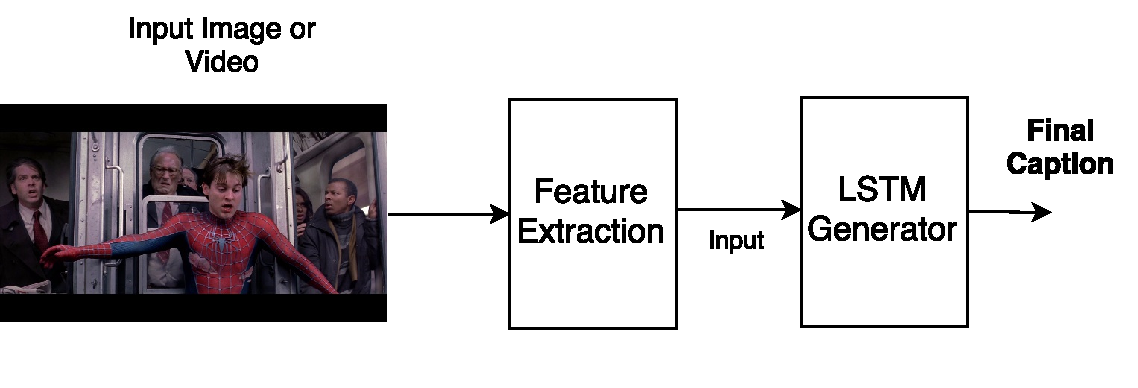
\includegraphics[width=0.8\linewidth]{images/Thesis_generalBaseline.pdf}
  \end{center}
  \vspace*{-8mm}
  \caption{A high-level block diagram of the visual captioning pipeline.}
  \label{fig_fullModel}
\end{figure}

\subsection{Visual Feature Extraction}

\paragraph{Baseline image feature.} As discussed in
Chapter~\ref{chapter:background}, image features extracted from CNNs pre-trained
on ImageNet have become ubiquitous in most image understanding tasks.
%%
Therefore, in our baseline captioning model we use features extracted from
GoogLeNet~\cite{DBLP:journals/corr/SzegedyLJSRAEVR14} as the image feature
vector.
%%
More details of the feature extraction process are discussed in
Chapter~\ref{chapter:VisFeatChapter}, but it suffices here to say that the feature
vectors are formed by the activations of the \emph{5th Inception module} in
GoogLeNet.
%%

\paragraph{Baseline video feature.} As a very simple baseline feature vector for
videos, we use the same GoogLeNet features as above, but extracted only from a
single key frame of the video.
%%
We choose the key frame as the frame at the center of the video's time-span.
%%
The idea behind using this simple feature vector is to enable the video
captioning baseline model to use the same pipeline as for images and to obtain a
reasonable baseline against which more sophisticated feature extraction methods
can be compared.

%%----------------------------------%%
\subsection{Language Model.}

The next stage in the pipeline is a conditional language model which
takes as input the visual features and generates a caption.
%%
The Long-Short Term Memory (LSTM) network~\cite{Hochreiter1997} architecture has
been a popular choice in the literature to model the probability of a sentence
$S$, given an visual feature $V$, as $P(S|V)$.
%%
The following two subsections contain a discussion of the LSTM cell in detail
and on the way it is used to build a conditional language model.

\subsubsection{LSTM Cell}

\begin{figure}[h]
  \begin{center}
    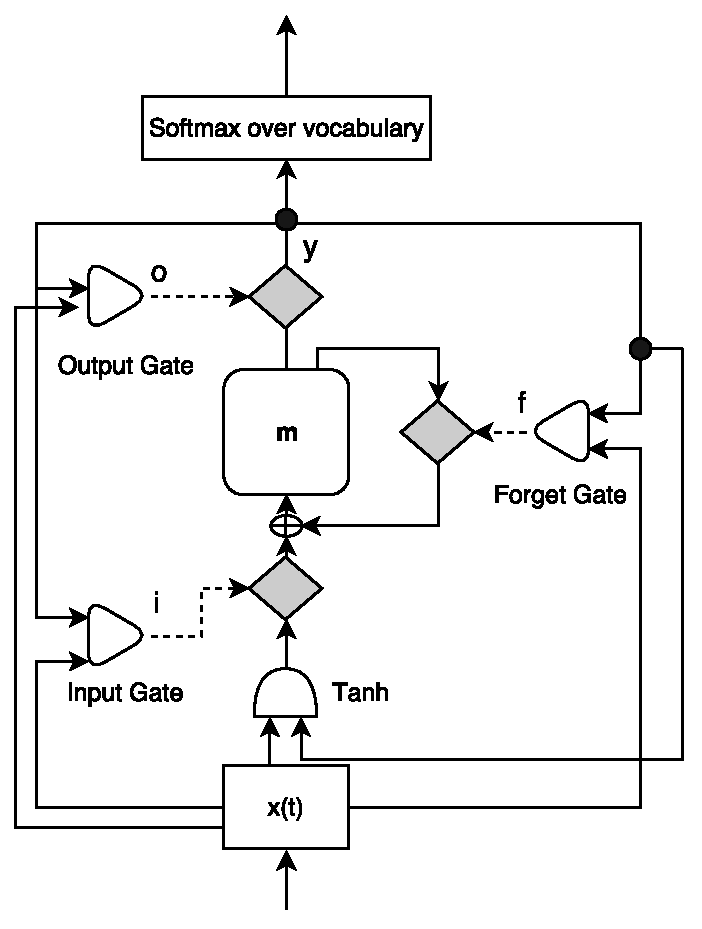
\includegraphics[width=0.5\linewidth]{images/LstmBlockDiag.pdf}
  \end{center}
  \vspace*{-6mm}
  \caption{A single LSTM cell. Dotted lines
    to the rhombi indicate multiplications as gate controls and the
    solid lines depict the data flow. The triangles are sigmoid
    non-linearities.}
  \label{fig:lstmcell}
\end{figure}

The LSTM model has been chosen as the language model based on two basic
requirements the image captioning problem imposes.
%%
Firstly, the language model needs to handle sentences of arbitrary length and
LSTMs are able to do this by design.
%%
Secondly, during the training with gradient descent methods, the error signal
and its gradients need to propagate a long way back in time without exploding,
and again LSTMs satisfy this criterion.

The block diagram of a single LSTM cell is shown in Figure~\ref{fig:lstmcell}.
%5
It consists of a memory cell $m$, whose value at any time step $t$ is influenced
by the current vectorial input $x(t)$, the previous output $y(t-1)$ and the
previous cell state $m(t-1)$.
%%
The update to the memory value $m$ is controlled using the input gate $i$ and
the forget gate $f$.
%%
The output is controlled using the output gate $o$.
%%
The gates are implemented with sigmoidal non-linearities $\sigma(\cdot)$ to keep
them completely differentiable.
%%

The input and forget gates of the LSTM cells have the ability to preserve the
content of the memory cell over long periods, which makes it easier to learn
longer sequences.
%%
This process is formalized in the equation system:
%%
\begin{align}
  \label{eqn:lstmstrt}
  i(t) &= \sigma(W_{ix}x(t-1) + W_{iy}y(t-1))\\
  o(t) &= \sigma(W_{ox}x(t-1) + W_{oy}y(t-1))\\
  f(t) &= \sigma(W_{fx}x(t-1) + W_{fy}y(t-1))\\
  \label{eqn:lstmend}
  \begin{split}
    m(t) &= f(t)\cdot m(t-1) \:\, + \\
    &\; \; \; \; \; i(t)\cdot \tanh(W_{mx}x(t)+W_{my}y(t-1))
  \end{split}\\
  y(t) &= o(t) \cdot m(t) \;,
\end{align}
%%
where $W_{\cdot\cdot}$ are the network weights learned during the
training phase.

%% --------------------------------------

\subsubsection{Basic LSTM Language Model}
\label{subsec:basiclstmodel}

The block diagram of the baseline language model is shown in
Figure~\ref{fig:baselinelstmlang}.
%%
The model consists of an LSTM network with a softmax layer at its output.
%%
The softmax outputs the probability distribution over the model's vocabulary as:
%%
\begin{align}
p(w_t | w_{t-1},\cdots,w_0, V) = \text{softmax}(D y(t)) \;,
\end{align}
\noindent where $D$ is the decoder matrix which maps the vector $y(t)$, with
the same dimensions as the number of LSTM units, to the output vocabulary size,
$Z$.
%%

The visual features $V$ are fed into the LSTM through an embedding matrix
$W_{ix}$ at the zeroth time step as the input $x(0)$.
%%
We refer to this feature input as the \emph{init} feature since it initializes
the hidden state of the LSTM.
%%
In the subsequent time steps $t$, a start symbol followed by the word embeddings
for each word in the reference caption (during training) or the previous
generated word (during testing) are fed through the same input line, as $x(t)$.

During the training phase, at each time step $t$, the LSTM is trained to assign
the highest probability to the next ground truth word given the current inputs
and the hidden state.
%%
This is done by maximizing the log likelihood assigned to the training samples
by the model.
%%
Equivalently, we can minimize the negative log likelihood given as
%%
\begin{align}
  \label{eqCost}
  \mathcal{NL}(w_0,\cdots, w_{L-1} | V) = -\sum_{t=0}^{L-1} \log(p(w_t|w_{t-1},V)) \; ,
\end{align}
\noindent where $w_{-1}$ is the start symbol and L is the length of the sentence.
%%
\begin{figure}[h]
\begin{center}
   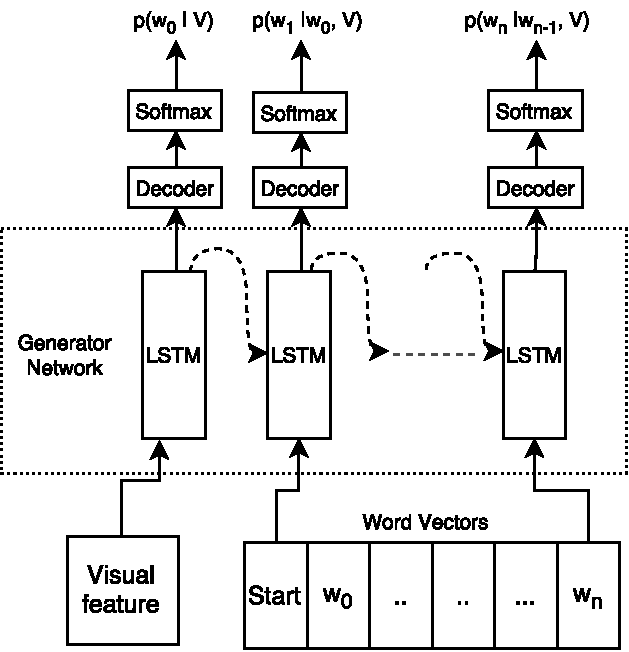
\includegraphics[width=0.5\linewidth]{images/Thesis_lstmLangGen.pdf}
\end{center}
\vspace*{-4mm}
\caption{The baseline LSTM-based language model with LSTMs unrolled in time.}
\label{fig:baselinelstmlang}
\end{figure}

\subsection{Training and Regularization}
%%----------------------------------%%
Training the network involves tuning the parameters of the language model in
order to minimize the negative log likelihood cost function shown in
(\ref{eqCost}).
%%
This optimization is achieved by backpropagating the cost through time and
adjusting the LSTM parameters using gradient descent.
%%
Specifically, stochastic gradient descent with the RMSProp~\cite{rmspropTielman}
algorithm is used.
%%
The training samples are used in random mini batches of sentence--image pairs,
and gradient descent is done after accumulating the cost for each mini batch.

All the LSTM parameters, the word embedding vectors and the decoder matrix are
learned using this method.
%%
The parameters of the feature extraction modules are not trained but are held
fixed in order to prevent overfitting.
%%
This is necessary as usually the feature extraction modules, e.g.\@ image CNN
network, are powerful models pre-trained on large datasets and can easily
overfit on the relatively small datasets such as the ones used in captioning.

Dropout is used for regularization during the training of the LSTM language
model.
%%
Dropout method, as the name suggests, involves randomly dropping the outputs
of some neurons in a layer to zero before feeding it to the next layer.
%%
This makes the neurons less co-dependent and more robust.
%%
As suggested in~\cite{ZarembaSV14}, the dropout is only applied on the input and
output of LSTM and not on the recurrent connections.
%%
We find that using dropout with a drop probability of $0.5$ greatly improves the
model generalization.
%%
Word embedding vectors and decoder matrix are regularized by adding a penalty to
minimize their $l_2$ norm.

\subsection{Test Mode: Beam Search}
%%
In the caption generation phase for test images, we do not have a reference
caption and need to sample from the distribution $P(S|I)$, to generate the
caption.
%%
Similar to the training phase, the image feature vector is fed into the LSTM
network at time-step $t=0$ followed by the `START' symbol.
%%
Then, at time-step $t=1$, the word with the highest probability at the softmax
output is the word the model thinks is the most likely first word.
%%
We pick it as the generated word and feed the corresponding word vector as the
input to the LSTM in the next time step, $t=2$.
%%
This iterative process is repeated until the model produces a period
symbol~(`.'), which marks the end of the generation process, and we have a
complete candidate sentence.
%%

One problem with this approach is that if we only consider the most likely word
at each time step we are not guaranteed to get the most likely final sentence.
%%
Ideally we should employ an approach akin to dynamic programming and search the
entire space of possible sentences.
%%
This is intractable as the space of all sentences, even with a finite
vocabulary, is infinite as sentences can be arbitrarily long.
%%
Even if we limit the sentence length, the search space still grows factorially
with the vocabulary size and is still too expensive to search exhaustively.
%%
A good approximation is to use beam search, wherein we maintain top $b$ partial
sentences at each step.
%%
For each of these top-$b$ sentences we consider extensions with top-$b$ words
and re-score the partial sentences.
%%
Of these $b^2$ possibilities only the best $b$ extensions are preserved.
%%
This process is repeated until all the search beams terminate or maximal
allowed sentence length is reached.
%%
At the end of this process we have $b$ generated candidate sentences ranked
according to the log likelihood assigned by the model.
%%

\section{Evaluation Metrics} \label{sec:EvaluationMetrics} The evaluation of
captioning systems is not trivial, due to the non-unique nature of the
solution space.
%%
An image can be correctly described with a wide variety of captions differing not
only in the syntactic structure, but also in the semantic content.
%%
We can see an example of this in Figure~\ref{fig_capdiversity}, where a sample
image from MS-COCO training set is shown with the corresponding ground truth
captions.
%%
We see that each caption focuses on different aspects of the image, from the
\emph{big rock} to \emph{crystal blue water}, but all the captions are equally
valid.
%%

A good method of evaluation is to compare the machine-generated caption with
multiple human-annotated reference captions.
%%
However, we need to note that the reference captions only represent few samples
from the space of all valid captions for the image.
%%
Having a large number of reference captions makes it more likely that the
solution space is better covered by them and thereby leading to more reliable
evaluation.
%%

\begin{figure}[t]
    \begin{minipage}[c]{0.45\linewidth}
        %\begin{center}
            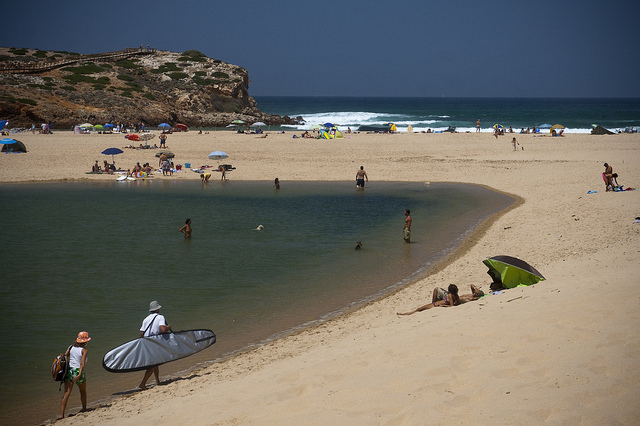
\includegraphics[width=\textwidth]{images/COCO_train2014_000000440903.jpg}
        %\end{center}
    \end{minipage}\hfill
    \begin{minipage}[c]{0.52\linewidth}
            \textbf{C1:} a beach with people relaxing on a \underline{sunny day}. \\
            \textbf{C2}: people are relaxing on the beach where there is a \underline{big rock}. \\
            \textbf{C3}: a beach with a group of people with surf boards and \underline{umberellas}. \\
            \textbf{C4}: a group of people enjoy a beach near a lagoon filled with \underline{crystal blue
            water}. \\
            \textbf{C5}: a \underline{man walking} on a beach with his surf board in a case. \\
    \end{minipage}
  \vspace*{-3mm}
  \caption{A sample image from the MS-COCO training set with associated ground
  truth captions. Here we see a clear case where different captions focus at
  least partially on different aspects of the image.}
  \label{fig_capdiversity}
\end{figure}

One aspect of the evaluation problem, the syntactic variations in target
sentences, is also seen in the well-studied field of machine translation.
%%
In this case, a sentence in one language could potentially be translated into
multiple valid sentences in the target language.
%%
Machine translation still differs from image captioning by the fact that,
although these multiple translations can differ syntactically, they tend to
have the same semantic content.

Nevertheless, image captioning literature has borrowed three evaluation metrics
popular in machine translation, namely BLEU~\cite{Papineni:BLEU},
ROUGE-L~\cite{lin2004rouge} and METEOR~\cite{denkowski-lavie:2014:Meteor}.
%%
Another metric popular in image captioning evaluation is the CIDEr metric which
was proposed recently in \cite{Vedantam_2015_CVPR}, specifically for this task.
%%
Next we will discuss each of these four metrics briefly to better understand
what exactly they measure.

\subsection{BLEU}

BLEU~\cite{Papineni:BLEU} is a simple metric which scores captions based on the
$n$-gram matches between the candidate and the reference captions.
%%
First, occurrence counts of different $n$-grams in the candidate sentence are
counted and clipped to their maximum value in any single reference sentence,
and then accumulated.
%%
Next, a modified precision score is computed by dividing this accumulated score
by the total number of $n$-grams in the candidate.
%%
This process is repeated for different n-grams, yielding modified precision
scores $p_n$.
%%
The final BLEU score is given by
\begin{equation}
    \text{BLEU-n} = BP\cdot{}\exp(\sum_{n=1}^{N}w_{n}\log(p_n)) \; ,
\end{equation}

\noindent where $BP$ is the brevity penalty applied in order to penalize
short candidate sentences.
%%
This additional term is required since, if we only use precision, degenerate
candidates such as the ones containing just single words will always score
better than longer sentences.
%%
\subsection{ROUGE-L}
ROUGE~\cite{lin2004rouge} metrics were proposed for evaluating text summaries.
%%
The version used in image captioning evaluation is ROUGE-L, a metric based on
recall and precision scores of the longest common subsequences~(LCS) between the
reference and candidate sentences:
%%
\begin{align}
        R_{lcs} &= \frac{LCS(Cand,Ref)}{Reference\ length} \; ,\\[0.75ex]
        P_{lcs} &= \frac{LCS(Cand,Ref)}{Candidate\ length} \; ,
\end{align}
%%
\noindent where $R_{lcs}$ and $P_{lcs}$ are recall and precision metrics,
$LCS(Cand,Ref)$ is the longest common subsequence between the candidate $Cand$ and reference
$Ref$.

The metric looks for common sub-sequences by looking for words which appear in the
same order in both the reference and candidate captions.
%%
Note that these words need not be consecutive, just in-sequence.
%%
Finally, the ROUGE-L metric is computed as the $F_\beta$ score with $\beta =
P_{lcs}/R_{lcs}$:

\begin{equation}
        \text{ROUGE-L} = F_{\beta} = \frac{(1+\beta^2)R_{ics}P_{lcs}}{R_{lcs}+ \beta^2 P_{lcs}} \; .
\end{equation}

\subsection{METEOR}
In order to compute the METEOR~\cite{denkowski-lavie:2014:Meteor} metric, the
candidate and reference sentences are first aligned, wherein each word in the
candidate sentence is matched to at most one word in the reference.
%%
When matching words between the candidate and the reference, apart from the
exact match, WordNet synonyms, stemmed token matches and paraphrase matches are
also considered, in that order.
%%
The alignment is done so as to minimize the number of chunks, i.e.\@ the group of
words which are consecutive and in order in both the sentences.
%%
Once the two sentences are aligned, weighted precision and recall are computed
on the matched words, with different weights being applied to different kinds of
matches.
%%
The final METEOR score is computed as the product of a penalty term to penalize the
number of chunks in the alignment and the F-score based on the weighted
precision and recall:
%%
\begin{align}
        Pen &= \gamma\cdot\left(\frac{ch}{m}\right)^\theta \; ,\\[0.75ex]
        \text{METEOR} &= (1-Pen)\frac{P_m R_m}{\alpha{}P_m+(1-\alpha)R_m} \; ,
\end{align}
%%
\noindent where $R_m$ and $P_m$ are the recall and precision metrics, $ch$ is
the number of chunks the alignment has, $m$ is the length of the candidate and
$\alpha$, $\gamma$ and $\theta$ are hyper-parameters tuned to maximize the
correlation of the metric with human judgment.
%%
When there are multiple references, the maximum METEOR score between the
candidate and any reference is taken.

\subsection{CIDEr}
CIDEr~\cite{Vedantam_2015_CVPR} metric aims to measure how well the candidate
caption matches with the consensus formed by the multiple reference captions.
%%
For this purpose, each candidate caption and reference sentence is represented
using term frequency inverse document frequency vectors (TF-IDF).
%%
TF represents the consensus, by considering frequently occurring terms in
the reference captions, and IDF helps down-weight common words which occur across
captions for many different images.

$\text{CIDEr}_n$ metric is computed by averaging the cosine similarity between
the TF-IDF vectors of the candidate caption and all reference captions.
%%
Here $n$ is the $n$-gram size considering which TF-IDF vector was formed.
%%
Final CIDEr metric is the mean of the four $\text{CIDEr}_n$ metrics, with $n=1,2,3,4$.
%%

Few modifications were made to this original CIDEr metric to prevent gaming,
i.e.\@ producing captions which could achieve higher CIDEr scores but fail badly
in human judgments.
%%
This is referred to as CIDEr-D and is the version widely used in image
captioning.

\subsection{Reliability of the Automatic Metrics}
\label{subsec:autMetRel}
In summary, all the four metrics discussed here evaluate the suitability of a
caption to the visual input, by comparing how well the candidate caption
matches the reference captions.
%%
They perform better with the increasing number of reference captions as was
found in~\cite{Vedantam_2015_CVPR}.
%%
The same study also found that CIDEr and METEOR have the highest correlations
to human judgment, followed by ROUGE-L and finally BLEU-4.
%%

All the four metrics were used to rank submissions in the first MS-COCO
image captioning challenge.
%%
The competition also collected human judgments to evaluate the submissions.
%
On comparing the two, it was found that the rankings produced by METEOR and
CIDEr were the ones most correlated with the ranking of submissions as per human
judgment~\cite{lsun2015CaptionSlides}, reaffirming the observations made
in~\cite{Vedantam_2015_CVPR}.
%%
Similar trend was also seen in the first Large-Scale Movie Description
Challenge~(LSMDC) 2015.
%%
The LSMDC 2015 used both the automatic metrics and the human judgments
to rank the submitted captions to the test videos.
%%
Even here, the ranking of the submissions produced by the automatic metrics
poorly correlated with the rankings produced by human judgments.

Hence in Chapter~\ref{chapter:results}, when evaluating the visual features and
language model architectures proposed in this thesis, most importance will be
given to METEOR and CIDEr metrics.
%%
We will also present results from human judgments of the video captioning
models presented in this thesis, obtained through participation in the LSMDC
2015 and the MSR-VTT challenges.

